%==============================
\subsection{Hardware Experiment}\label{subsec:hardware-experiment}
For further validation with hardware,
a similar set-up as the simulation is built as shown in Fig.~\ref{fig:ws}.
In total~$4$ UAVs and $2$ UGVs are deployed in the workspace of of $4\times5\, m^2$.
Each robot communicates wirelessly to the control PC via ROS,
of which the state is monitored by the OptiTrack system.
Different tasks and scenarios are designed to show
how the proposed methods perform on actual hardware.
Experiment videos can be found in the supplementary file.


%==============================
\begin{figure}[t!]
  \begin{minipage}[t]{0.49\linewidth}
    \centering%
	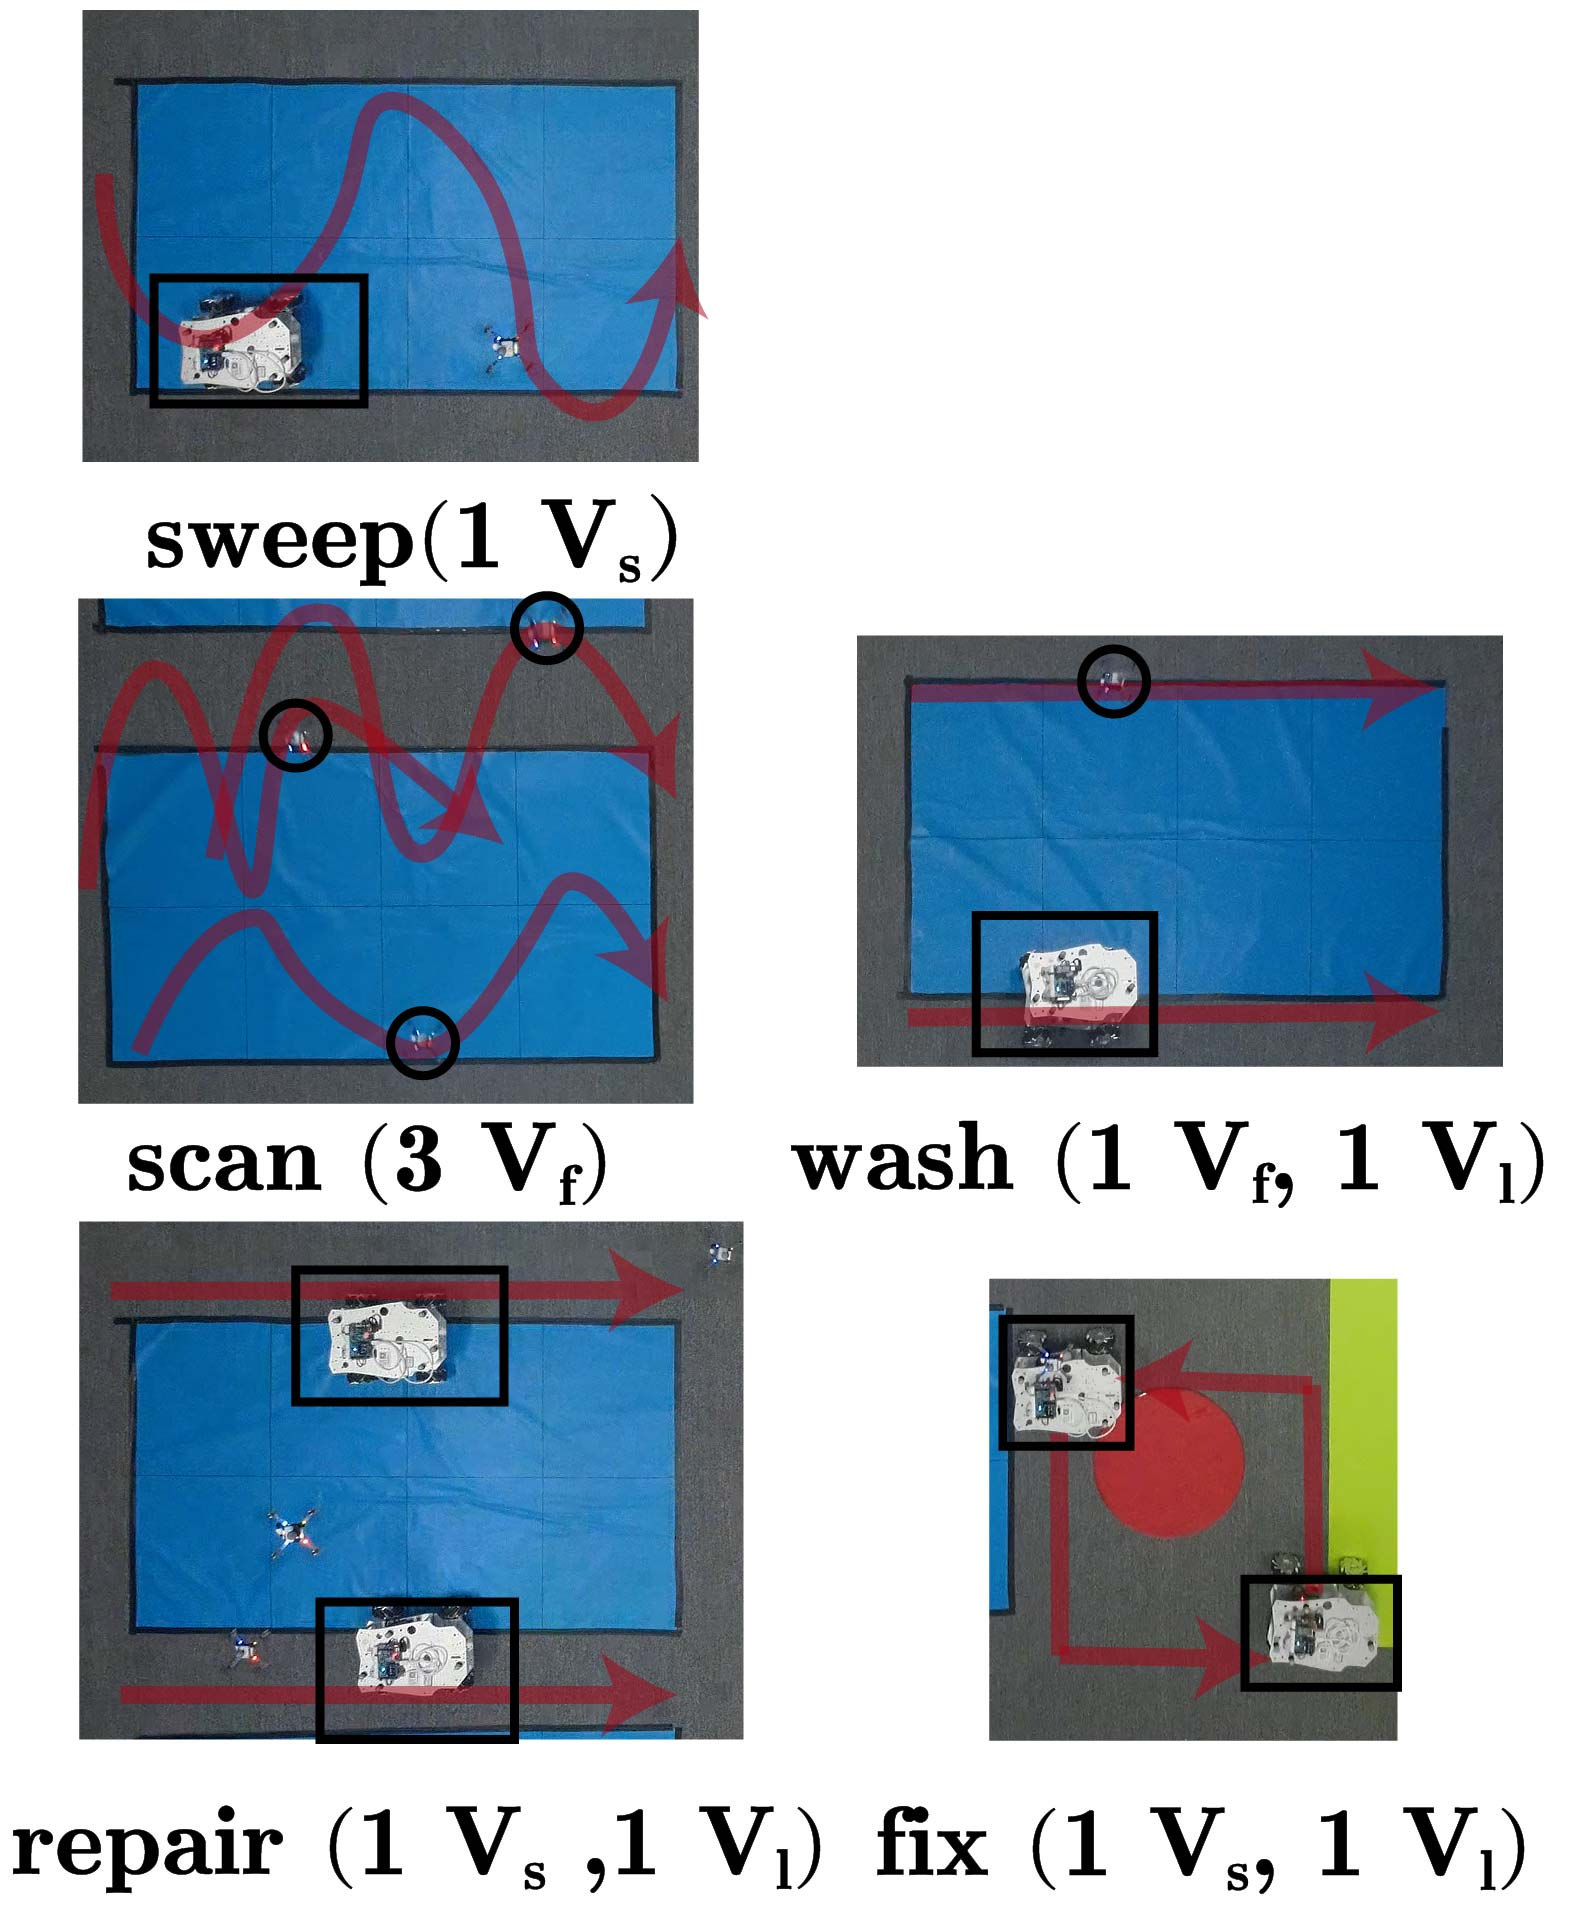
\includegraphics[width =0.88\textwidth]{figures/hardware_experiment/washing.jpg}
\end{minipage}%
  \begin{minipage}[t]{0.49\linewidth}
    \centering
	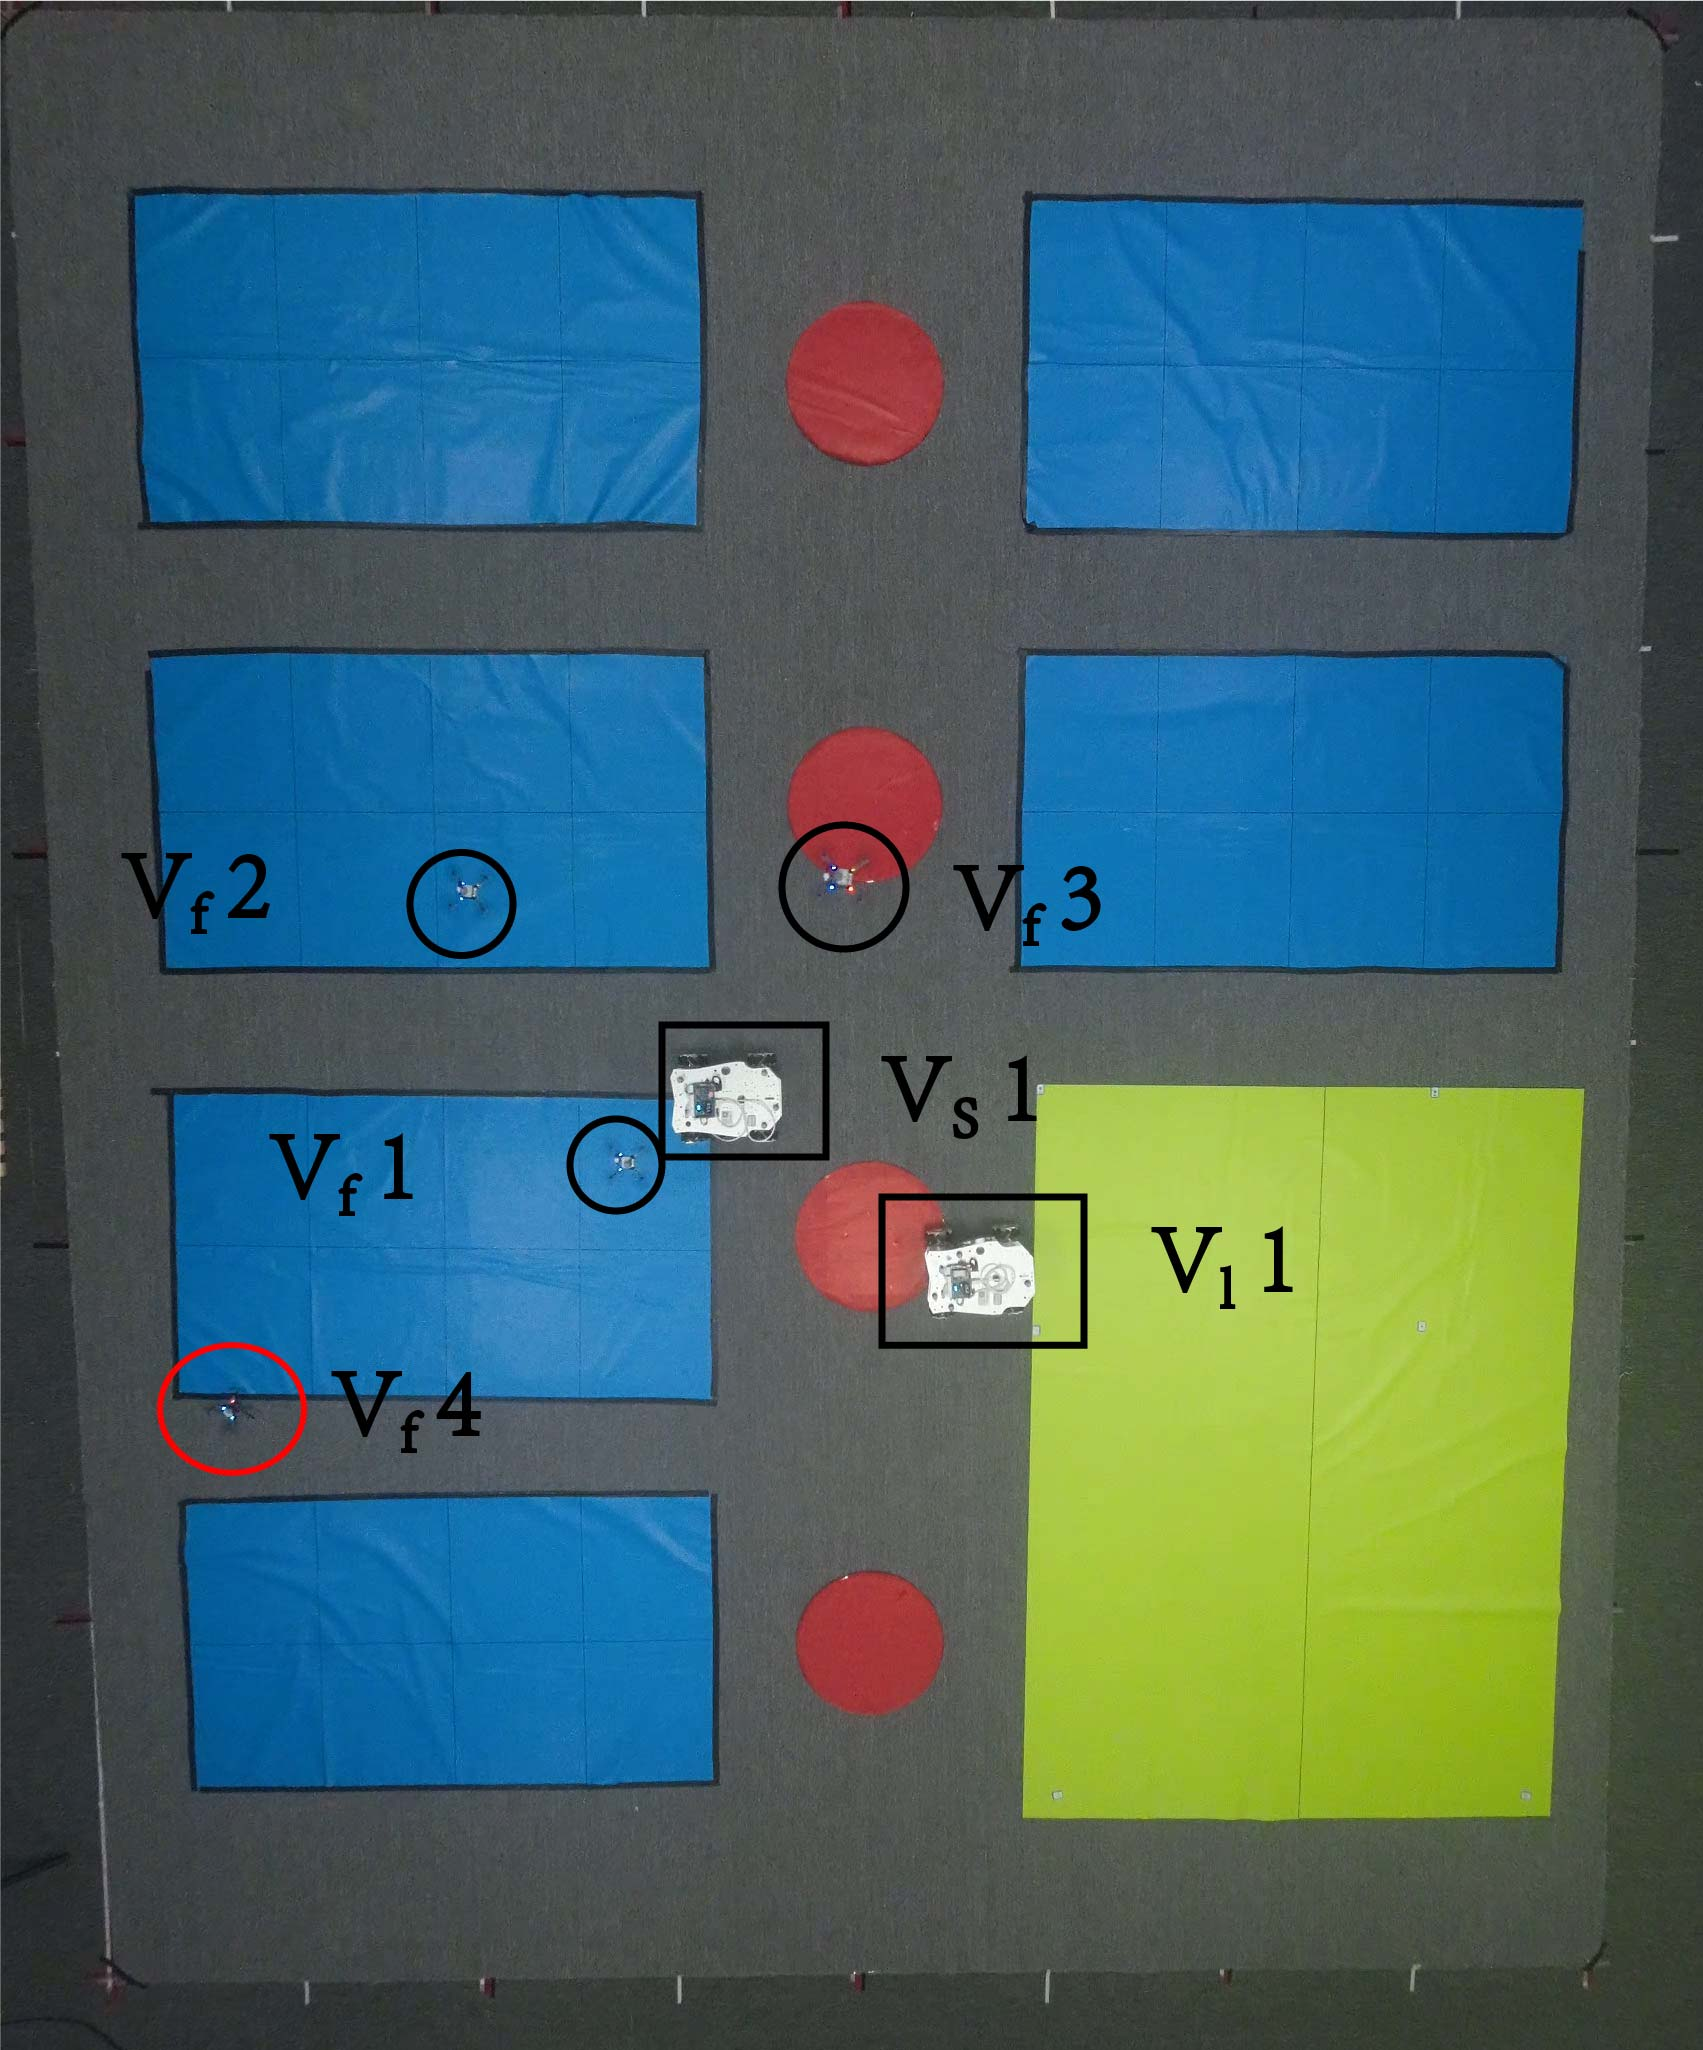
\includegraphics[width =0.9\textwidth]{figures/hardware_experiment/experiment2.jpg}
\end{minipage}%
\caption{Snapshots of the task execution. \textbf{Left}:
Trajectory and collaborators of subtasks.
\textbf{Right}: UAV $4$ (marked in red) is manually stopped to mimic motor failure,
while the rest of the team adapts and continues
the task execution.}
\label{fig:ws}
\end{figure}
%==============================

The workspace mimics the PV farm described in the numerical simulation.
As showed in Fig.~\ref{fig:ws},
there are~$6$ PV panels ($\texttt{p}_1$-$\texttt{p}_6$, marked in blue),
$4$ transformer substations
($\texttt{t}_1$-$\texttt{t}_4$, marked in red)
and~$1$ base station ($b_1$ marked in yellow).
Moreover,~$4$ UAVs and~$2$ UGVs are deployed to maintain the PV farm,
where the UAVs are Crazyfly mini-drones (denoted by~$V_f$) and
the UGVs are four-wheel driven cars with mecanum wheels (denoted by~$V_s$, $V_l$).
Existing mature navigation controllers are used and omitted here for brevity.
The routine maintenance task considered can be specified with the following LTL formulas:
\begin{equation}\scriptsize
\begin{aligned}
	\varphi_4=& \Diamond(\texttt{repair}_{\texttt{p}_2} \land  \lnot\texttt{scan}_{\texttt{p}_2} \land \Diamond
	\texttt{scan}_{\texttt{p}_2} \land \Diamond (\texttt{sweep}_{\texttt{p}_2} \land \texttt{repair}_{\texttt{p}_2}) )\\ 
	& \land \Diamond \texttt{fix}_{\texttt{t}_1} \land \Diamond \texttt{scan}_{\texttt{p}_3}
	\land \Diamond \texttt{wash}_{\texttt{p}_5}
\end{aligned}
\end{equation}


The proposed algorithm are successfully executed, following the procedure described in Alg.~\ref{alg:complete},
the LTL formula is converted to its NBA~$\mathcal{B}$ with $62$ nodes and $521$ edges.
And the pruned NBA~$\mathcal{B}^-$ has $62$ nodes and $377$ edges.
Only one poset is found with Alg.~\ref{alg:compute-poset},
which contains~$6$ subtasks whose language~$L(P)$ equals to the full language~$L(\mathcal{B}^-)$.
Furthermore, Alg.~\ref{alg:upper_bound} finds the
optimal task assignment within~$3.7s$,
which has the estimated makespan of~$124s$, after exploring~$59$ nodes.
Moreover, to test the online adaptation procedure
as described in Sec.~\ref{subsubsec:failure},
one UAV~$V_{f_4}$ is stopped manually to mimic a motor failure during execution at~$75s$
 and a new plan is found within~$0.8s$.
As a result, UAV~$V_{f_1}$ takes over the subtask~$\texttt{scan}_{\texttt{P}_2}$
to continue the overall mission. 

 

